% SPDX-FileCopyrightText: Copyright (c) 2023 Yegor Bugayenko
% SPDX-License-Identifier: MIT

\documentclass{article}
\usepackage[T1]{fontenc}
\usepackage[utf8]{inputenc}
\usepackage[nocn,nonumbers,noframes,sf,bold]{ffcode}
\usepackage[static]{clicks}
\usepackage{tikzsymbols}
\usetikzlibrary{positioning}
\usepackage[increment]{crumbs}
\usepackage[template,scheme=light,nominutes]{ppt-slides}
\usepackage{href-ul}
\usepackage{svg}
\usepackage{soul}
\usepackage{qrcode}
\renewcommand{\ttdefault}{cmtt}
\newcommand\nospell[1]{#1}
\newcommand*{\thetitle}{Welcome to R\&D}
\newcommand*{\thesubtitle}{How Much of It You Can Afford?}
\newcommand*{\theauthor}{Yegor Bugayenko}
\pptLeft{}
\pptRight{@yegor256}

\renewcommand\emph[1]{\ul{#1}}

\begin{document}

\plush{
  \begin{pptMiddle}
    % 
\includegraphics[height=1.6in]{logo.png}
    \pptTitle{\thetitle}{\thesubtitle}\par
    {\scshape \theauthor}
    \newline
    {\small Huawei Technologies Co., Ltd.\par}
  \end{pptMiddle}
}

\plush{\pptThought{What is R\&D?}}

\plush{\pptThought{Research and development are very difficult to manage, since the defining feature of research is that the researchers \emph{do not know} in advance exactly how to accomplish the desired result. --- Wikipedia}}

\plush{
  \pptBanner{Challenge \#1: Goal Setting}
  \begin{multicols}{2}
  The goal must be:
  \begin{itemize}
    \item Global / Ambitious
    \item Hard to achieve
    \item Ego-friendly
    \item Business-friendly
  \end{itemize}
  \par\columnbreak\par
  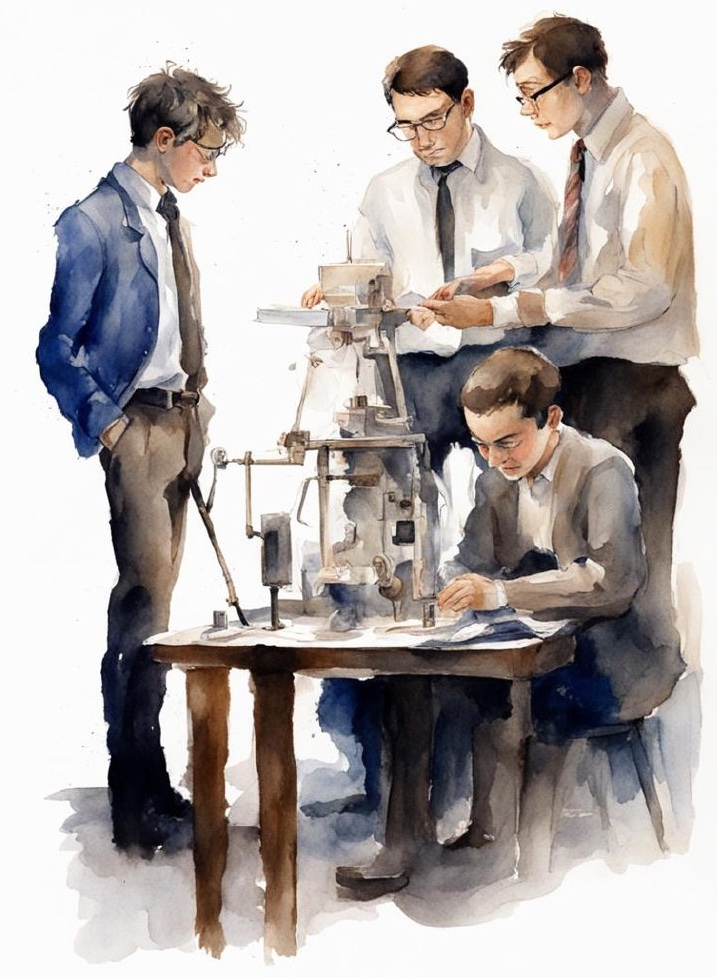
\includegraphics[width=.7\columnwidth]{goal-setting.jpg}
  \end{multicols}
}

\plush{
  \pptBanner{Challenge \#2: Decomposition \& Planning}
  \begin{multicols}{2}
  Possible work packages:
  \begin{itemize}
    \item Research paper
    \item Patent
    \item Tech Report
    \item Seminar
  \end{itemize}
  \par\columnbreak\par
  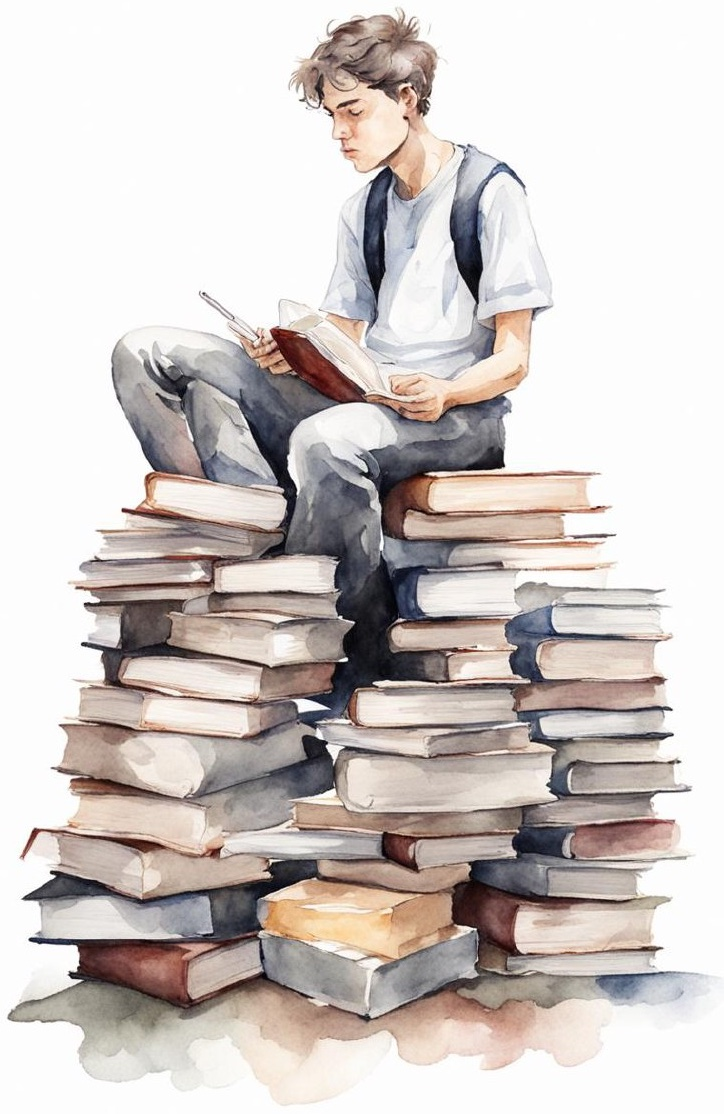
\includegraphics[width=.65\columnwidth]{decomposition.jpg}
  \end{multicols}
}

\plush{
  \pptBanner{Challenge \#3: Metrics \& KPI}
  \begin{multicols}{2}
  Possible metrics:
  \begin{itemize}
    \item ACM Journal Paper: +50
    \item ACM A* Conference: +10
    \item ACM/IEEE Conference: +5
    \item Patent: +5
  \end{itemize}
  \par\columnbreak\par
  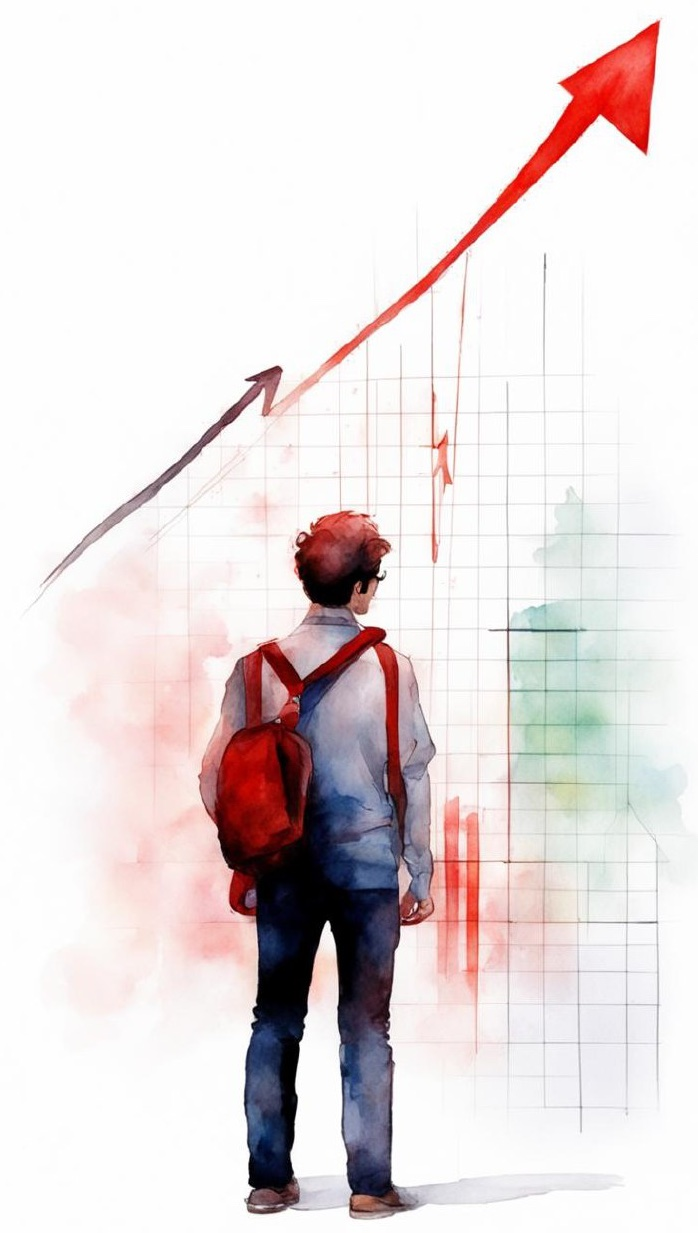
\includegraphics[width=.55\columnwidth]{kpi.jpg}
  \end{multicols}
}

\plush{
  \pptBanner{Challenge \#4: Embrace the Failure}
  \begin{multicols}{2}
  When we fail, we:
  \begin{itemize}
    \item Prove
    \item Learn
    \item Help others
    \item Boost H-Index
  \end{itemize}
  \par\columnbreak\par
  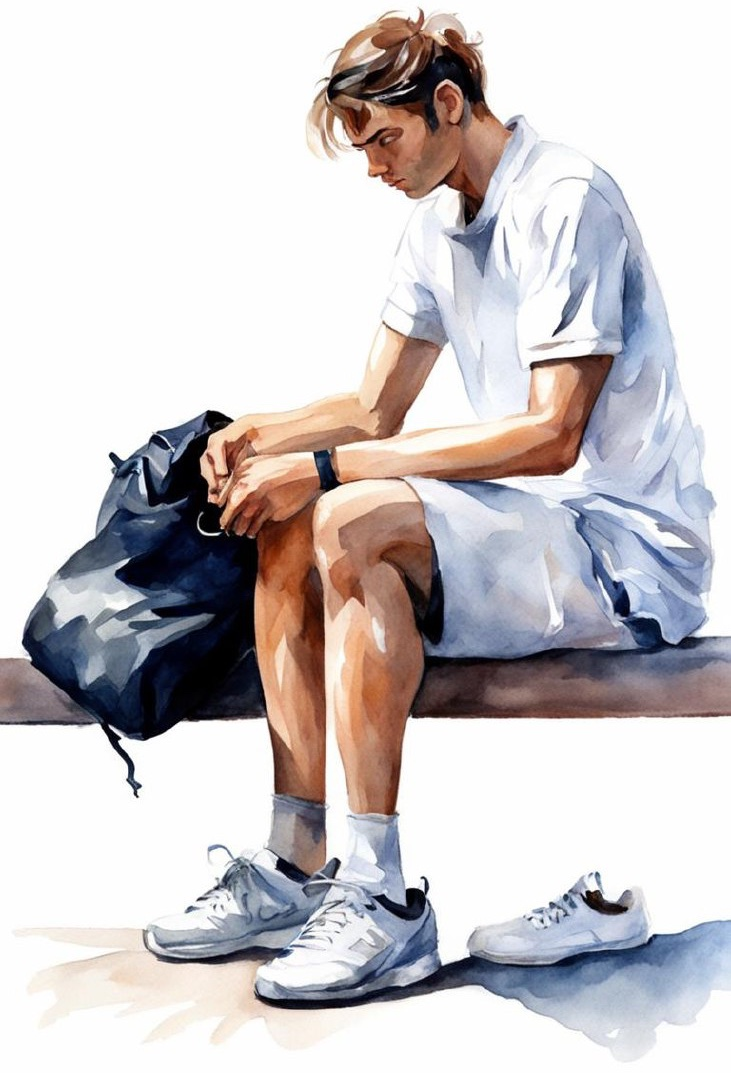
\includegraphics[width=.6\columnwidth]{failure.jpg}
  \end{multicols}
}

\plush{\pptBanner{My Telegram Channel:}\qrcode[height=3in]{https://t.me/yegor256news}\par\texttt{@yegor256news}\par
  {\small BTW, all pictures are made by \href{https://t.me/kandinsky21_bot}{Kandinsky 3.0 Telegram Bot}\par}}

\end{document}
